\documentclass{article}
\usepackage[utf8]{inputenc}
\usepackage[margin=0.8in]{geometry}
\usepackage{graphicx}
\usepackage{wrapfig}

\usepackage{natbib}
\usepackage{graphicx}
% Para los codigos
\usepackage{listings}
\usepackage[spanish]{babel}
\usepackage[hidelinks]{hyperref}


\begin{document}

\begin{titlepage}
	\title{
		\begin{Huge}
			Practica 1 + 2 - BASES DE DATOS 2
		\end{Huge}
	}
	\author{
	  Hayk Kocharyan\\
	  757715@unizar.es
	  \and
	  Pedro Tamargo Allué\\
	  758267@unizar.es
	  \and
	  Jesús Villacampa Sagaste\\
	  755739@unizar.es
	  \and
	  Juan José Tambo Tambo\\
	  755742@unizar.es
	}
	\date{\today}
	
	\clearpage\maketitle
	\thispagestyle{empty}
	\tableofcontents
	\listoffigures 
	
\end{titlepage}

\newpage 

\section{Esfuerzos invertidos}
Los esfuerzos invertidos por cada integrante del equipo son:
\begin{itemize}
\item Hayk:
\item Juan:
\item Jesús:
\item Pedro: 
\end{itemize}

\section{Configuración de la máquina virtual}
Para la realización de esta práctica se han utilizado las máquinas de 32 y 64 bits y su configuración ha sido igual para ambas.\\

Para la instalación de los \emph{SGBD} se debía conectar por medio de ssh  desde la máquina local utilizando $ssh -X root@dirmaquina$ para poder utilizar herramientas gráficas necesarias. Para ello, se debe configurar las interfaces de red de las máquinas de la siguiente manera:\\
Desde VirtualBox, añadir un adaptador “Host-only Adapter”:\\
$Configuracion->Network->Adapter2->Host-only Adapter (Name: vboxnet0).$
\\
Para que aparezca vboxnet0:\\
$File->Host Network Adapter->create$
\\
Una vez realizado lo anterior, desde la máquina virtual, se debe configurar el archivo /etc/network/interfaces y modificar la interfaz eth1 de la manera ilustrada en la Figura \ref{FIG:interfacesRED}.


\section{Instalación y administración básica de los SGBD}

En la instalación de los \emph{SGBD} se ha creado un usuario para la administración de la base de datos.\\
Para la base de datos Oracle se ha creado un usuario \emph{oracle}. En especial en la instalación de este \emph{SGBD} ha sido problematica en la instalación. Existen problemas con el espacio de la máquina. Al instalar todos los gestores no quedaba sitio suficiente para instalar Oracle.\\
Para arreglar este problema se ha aumentado el espacio del disco proporcionado con la máquina a 32GB. Pero al intentar aumentar la particion (/dev/sda1)
que estaba montada en / hemos notado que existía una partición swap (/dev/sda5) que nos impedía redimensionar la primera.\\
Para intentar solucionar este problema se creó el nuevo espacio adicional como otra partición (/dev/sda3) y editando el fichero /etc/fstab se montó en el arranque
en el directorio /oracle, directorio home del usuario oracle (necesario para la instalacion del SGBD).\\
Esto solucionó el problema con el espacio, pero tras proseguir con la instalación nos encontramos con un apartado de comprobación de prerrequisitos. Aquí se comprueban
de manera automática que se cumplen ciertas precondiciones. Nuestra máquina no las cumplía y, el instalador propone como solución ejecutar un script ubicado en el directorio
/tmp.\\
Al intentarlo ejecutar la terminal nos muestra ciertos errores de formateo:

\begin{lstlisting}[language=bash]
	./orarun.sh: 186: [: true: unexpected operator
	./orarun.sh: 186: [: true: unexpected operator
	./orarun.sh: 848: [: unexpected operator
	./orarun.sh: 864: [: unexpected operator
	./orarun.sh: 882: [: unexpected operator
	./orarun.sh: 903: [: true: unexpected operator
	./orarun.sh: 1052: [: unexpected operator
	./orarun.sh: 1057: [: unexpected operator
	./orarun.sh: 1075: [: unexpected operator
	./orarun.sh: 1085: [: unexpected operator
	./orarun.sh: 1115: [: unexpected operator
	./orarun.sh: 1143: [: unexpected operator
	./orarun.sh: 1189: [: unexpected operator
	./orarun.sh: 139: [: unexpected operator
	./orarun.sh: 139: [: unexpected operator
	./orarun.sh: 1228: [: unexpected operator
	./orarun.sh: 1284: [: unexpected operator
	./orarun.sh: 1342: [: unexpected operator
	./orarun.sh: 1426: [: unexpected operator
	./orarun.sh: 1451: [: unexpected operator
\end{lstlisting}

Al inspeccionar el archivo orarun.sh no se encuentra ningún problema. Al buscar en Internet la única explicación que se encuentra es que estamos instalando
Oracle en una distro no certificada para ello.
Por ello procedemos a instalar Oracle en la máquina de 32 bits.\\

En la instalación de \emph{PostgreSQL} procedemos a instalar la versión \emph{9.6}, para ello ejecutamos la orden: \\

\begin{lstlisting}[language=bash]
    sudo apt -y install postgresql-9.6
\end{lstlisting}

Se habrá creado el usuario \emph{postgres}. Para la interacción con la base de datos iniciaremos sesión como este usuario. Para ello ejecutaremos:

\begin{lstlisting}
    sudo su - postgres
\end{lstlisting}

Para iniciar el shell interactivo de postgre utilizaremos $psql postgres$. Si queremos crear una base de datos ejecutaremos:
\begin{lstlisting}
    createdb <nombre_base_datos>
\end{lstlisting}

En el caso de que no se encuentre el binario ejecutaremos el mismo utilizando la ruta absoluta

\begin{lstlisting}
    /usr/local/pgsql/bin/createdb <nombre_base_datos>
\end{lstlisting}

\emph{PostgreSQL} utiliza metacomandos para interactuar con su shell interactivo. El listado de metacomandos se puede encontrar aquí\footnote{\url{https://dataschool.com/learn-sql/meta-commands-in-psql/}}.\\

Para la instalación de \emph{DB2} descargaremos los ficheros desde \url{https://jazz.net/downloads/DB2/releases/10.1}, utilizaremos la versión \emph{Linux x86-64}. Una vez descargado, extraeremos el fichero con la órden:

\begin{lstlisting}
    tar -xzvf <filename> .
\end{lstlisting}

Una vez descomprimido accederemos al directorio y ejecutaremos la orden:

\begin{lstlisting}
    sudo ./db2_setup
\end{lstlisting}

Crearemos un usuario.\\
Añadiremos el directorio a la variable de entorno \emph{PATH} modificando nuestro fichero $~/.profile$.\\
Para crear una nueva instancia de \emph{DB2} ejecutaremos:

\begin{lstlisting}
    db2ictr <nombre_instancia>
\end{lstlisting}

Seleccionaremos la nueva instancia como la instancia por defecto utilizando:

\begin{lstlisting}
    set db2instance=<nombre_instancia>
\end{lstlisting}

Ahora todas las acciones se ejecutarán sobre esa instancia.
Debemos cambiar de usuario al creado anteriormente.
\begin{lstlisting}
    su - <nombre_usuario>
\end{lstlisting}

Para crear una base de datos ejecutaremos:
\begin{lstlisting}
    db2 create database <database_name>
\end{lstlisting}

Iniciamos la base de datos:
\begin{lstlisting}
    db2start
\end{lstlisting}

Para conectarnos a la base de datos que hemos creado escribiremos:
\begin{lstlisting}
    db2 connect to <database_name>
\end{lstlisting}

Para crear una tabla podemos hacerlo desde fuera del shell de DB2 escribiendo:
\begin{lstlisting}
    db2 create table prueba(id integer not null primary key)
\end{lstlisting}

Para mostrar las tablas escribiremos:
\begin{lstlisting}
    db2 list tables
\end{lstlisting}

Con \emph{db4o}, un \emph{SGBD} orientado a objetos, no se requiere instalación ya que se ejecuta desde un fichero \emph{.jar} proporcionado junto con el enunciado de la práctica.

\section{Comentarios acerca de las licencias}

\begin{Huge}
	¿RELLENAMOS ESTO CON \LaTeX?
\end{Huge}

\section{Diseño conceptual de la base de datos}

Para el diseño de la Base de Datos especificada en el enunciado se ha utilizado el siguiente diagrama entidad relación (Figura \ref{FIG:diagramaER}).

También para facilitar el diseño de la base de datos orientada a objetos utilizando \emph{db4o} se ha creado un diagrama de clases \emph{UML} (Figura \ref{FIG:diagramaUML}).



\section{Diseño lógico de una base de datos relacional}

\subsection{Implementación con el modelo relacional}

Para la transformación del del Diagrama Entidad-Relación en un modelo relacional se ha convertido la generalización de Cuenta en dos tablas, sus subtablas $Cuenta\_ahorro$ y $Cuenta\_corriente$, y la generalización de Transacción en sus dos subtablas Transferencia y Operación.\\

Las relaciones entre las entidades se han traducido en función de su cardinalidad. Las relaciones \emph{(M:N)} se han traducido en una nueva relación.\\

\textbf{Para la implementación en el SGBD Oracle se han utilizado tablas las tablas especificadas anteriormente y se han establecido las restricciones de integridad referencial a las tablas que hacen referencia a otras. ??}

Por lo tanto, podremos convertir el Diagrama Entidad-Relación (Figura \ref{FIG:diagramaER}) en el Diagrama Relacional (Figura \ref{FIG:diagramaRel}).

\section{Diseño lógico de una base de datos objeto/relacional}
\subsection{Implementación con el modelo objeto/relacional}
\subsubsection{Oracle}
Para la implementación del modelo \emph{OR} con \emph{Oracle} se han creado tantos tipos como entidades teníamos en el Diagrama Entidad-Relación, además para reflejar las relaciones bidireccionales entre dos entidades se han creado otros tipos (listaCuentas, listaPropietarios y realizadasUdt) como tablas de referencias a otros tipos ya creados anteriormente.
\\
Tras la creación de los tipos, procedemos a crear las tablas de los mismos. Oracle tiene como particularidad que no existen jerarquías de tablas, es decir, crearemos una tabla para el supertipo de la jerarquía y realizaremos las restricciones de integridad referencial mediante las cláusulas \emph{FOREIGN KEY} en las tablas y \emph{SCOPE} en las tablas anidadas.
\\

\subsubsection{PostgreSQL}

Para la implementación del modelo \emph{OR} utilizando \emph{PostgreSQL} se ha maximizado el uso de la herencia de tablas como mecanismo de relación entre las distintas entidades planteadas en el diagrama \emph{ER} (Figura \ref{FIG:diagramaER}).\\
Para la traducción de las relaciones \emph{M:N} se han creado entidades específicas ya que, a pesar de que si se han utilizado referencias, en este gestor la propiedad del modelo OR que se ha buscado explotar es la herencia. Otros gestores como Oracle no la poseen y en el diseño referente a este gestor ya se han explotado otras características como son los tipos, tablas tipadas o arrays, por tanto no se considera primordial explotarlas también en PostgreSQL y centrar esfuerzos en observar todo lo que ofrece la herencia.\\
Se han observado ciertas limitaciones a la hora de la realización de pruebas, mediante inserciones y consultas que se explican en el propio documento de pruebas a través de comentarios.\\
\\

\subsubsection{DB2}

Para la implementación con \emph{DB2} se ha seguido un planteamiento muy similar al de \emph{Oracle}. Se han creado tipos (\emph{UDT}) para las distintas entidades del Diagrama Entidad-Relación (Figura \ref{FIG:diagramaER}). Tras la creación de los tipos de datos se han creado las tablas tipadas.\\
A diferencia de \emph{Oracle}, este \emph{SGBD} tiene la capacidad de permitir la herencia entre tablas. De esta forma se han creado tantas tablas como tipos se han definido anteriormente.\\
Una diferencia con 
\begin{Large}
	(Comprobar si esto es así)
\end{Large}
el estándar \emph{SQL:1999} la cláusula \emph{SCOPE} no garantiza la integridad referencial entre las tablas, por lo tanto se deben utilizar restricciones de clave ajena (\emph{Foreign key}) para garantizarla\footnote{\url{https://www.ibm.com/support/knowledgecenter/SSEPGG_11.5.0/com.ibm.db2.luw.admin.structypes.doc/doc/c0006594.html}}.
\\

\section{Generación de datos y pruebas}

Para la generación de datos y la realización de pruebas se han creado conjuntos de datos para la población y las pruebas de las distintas bases de datos con los gestores seleccionados.\\

Para la generación de datos, se han utilizado generadores de códigos de cuenta bancaria e IBAN. Los DNIs y los nombres han sido inventados por los integrante del equipo.

Se han probado consultas que recorrían las relaciones entre las entidades, resolviendo las referencias que aparecían entre las mismas.
%\textbf{\Huge RELLENAR ESTO MÁS}

\section{Implementación con db4o}

Siguiendo el diagrama \emph{UML} de la Figura \ref{FIG:diagramaUML}, se ha procedido a la creación de las clases \emph{Java} correspondientes. A diferencia de la implementación en el modelo relacional de \emph{Oracle}, no es necesario reflejar las relaciones \emph{M:N} como una nueva entidad, en este caso se utilizarán listas (\emph{List}).\\

Una de las dificultades encontradas en la implementación con \emph{db4o} ha sido el desfase entre versiones de \emph{Java}, por ejemplo en el uso de clases genéricas ya que la Máquina Virtual de \emph{Java} mostraba avisos (\emph{Warnings}) acerca de la instanciación de las clases.

Para la resolución de las dudas surgidas durante la implementación con este \emph{SGBD} se ha recurrido al manual del mismo\footnote{\url{http://www.odbms.org/wp-content/uploads/2013/11/db4o-7.10-tutorial-java.pdf}}.

\section{Comparación de los SGBD}

\newpage
\section{Apéndice 1: Figuras}

\begin{figure}[h!]
	\centering
		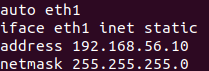
\includegraphics[scale=1.5]{images/interfacesred.png}
			\caption{Interfaz de red para el acceso vía SSH}
		\label{FIG:interfacesRED}
\end{figure}

\begin{figure}[h!]
	\centering
		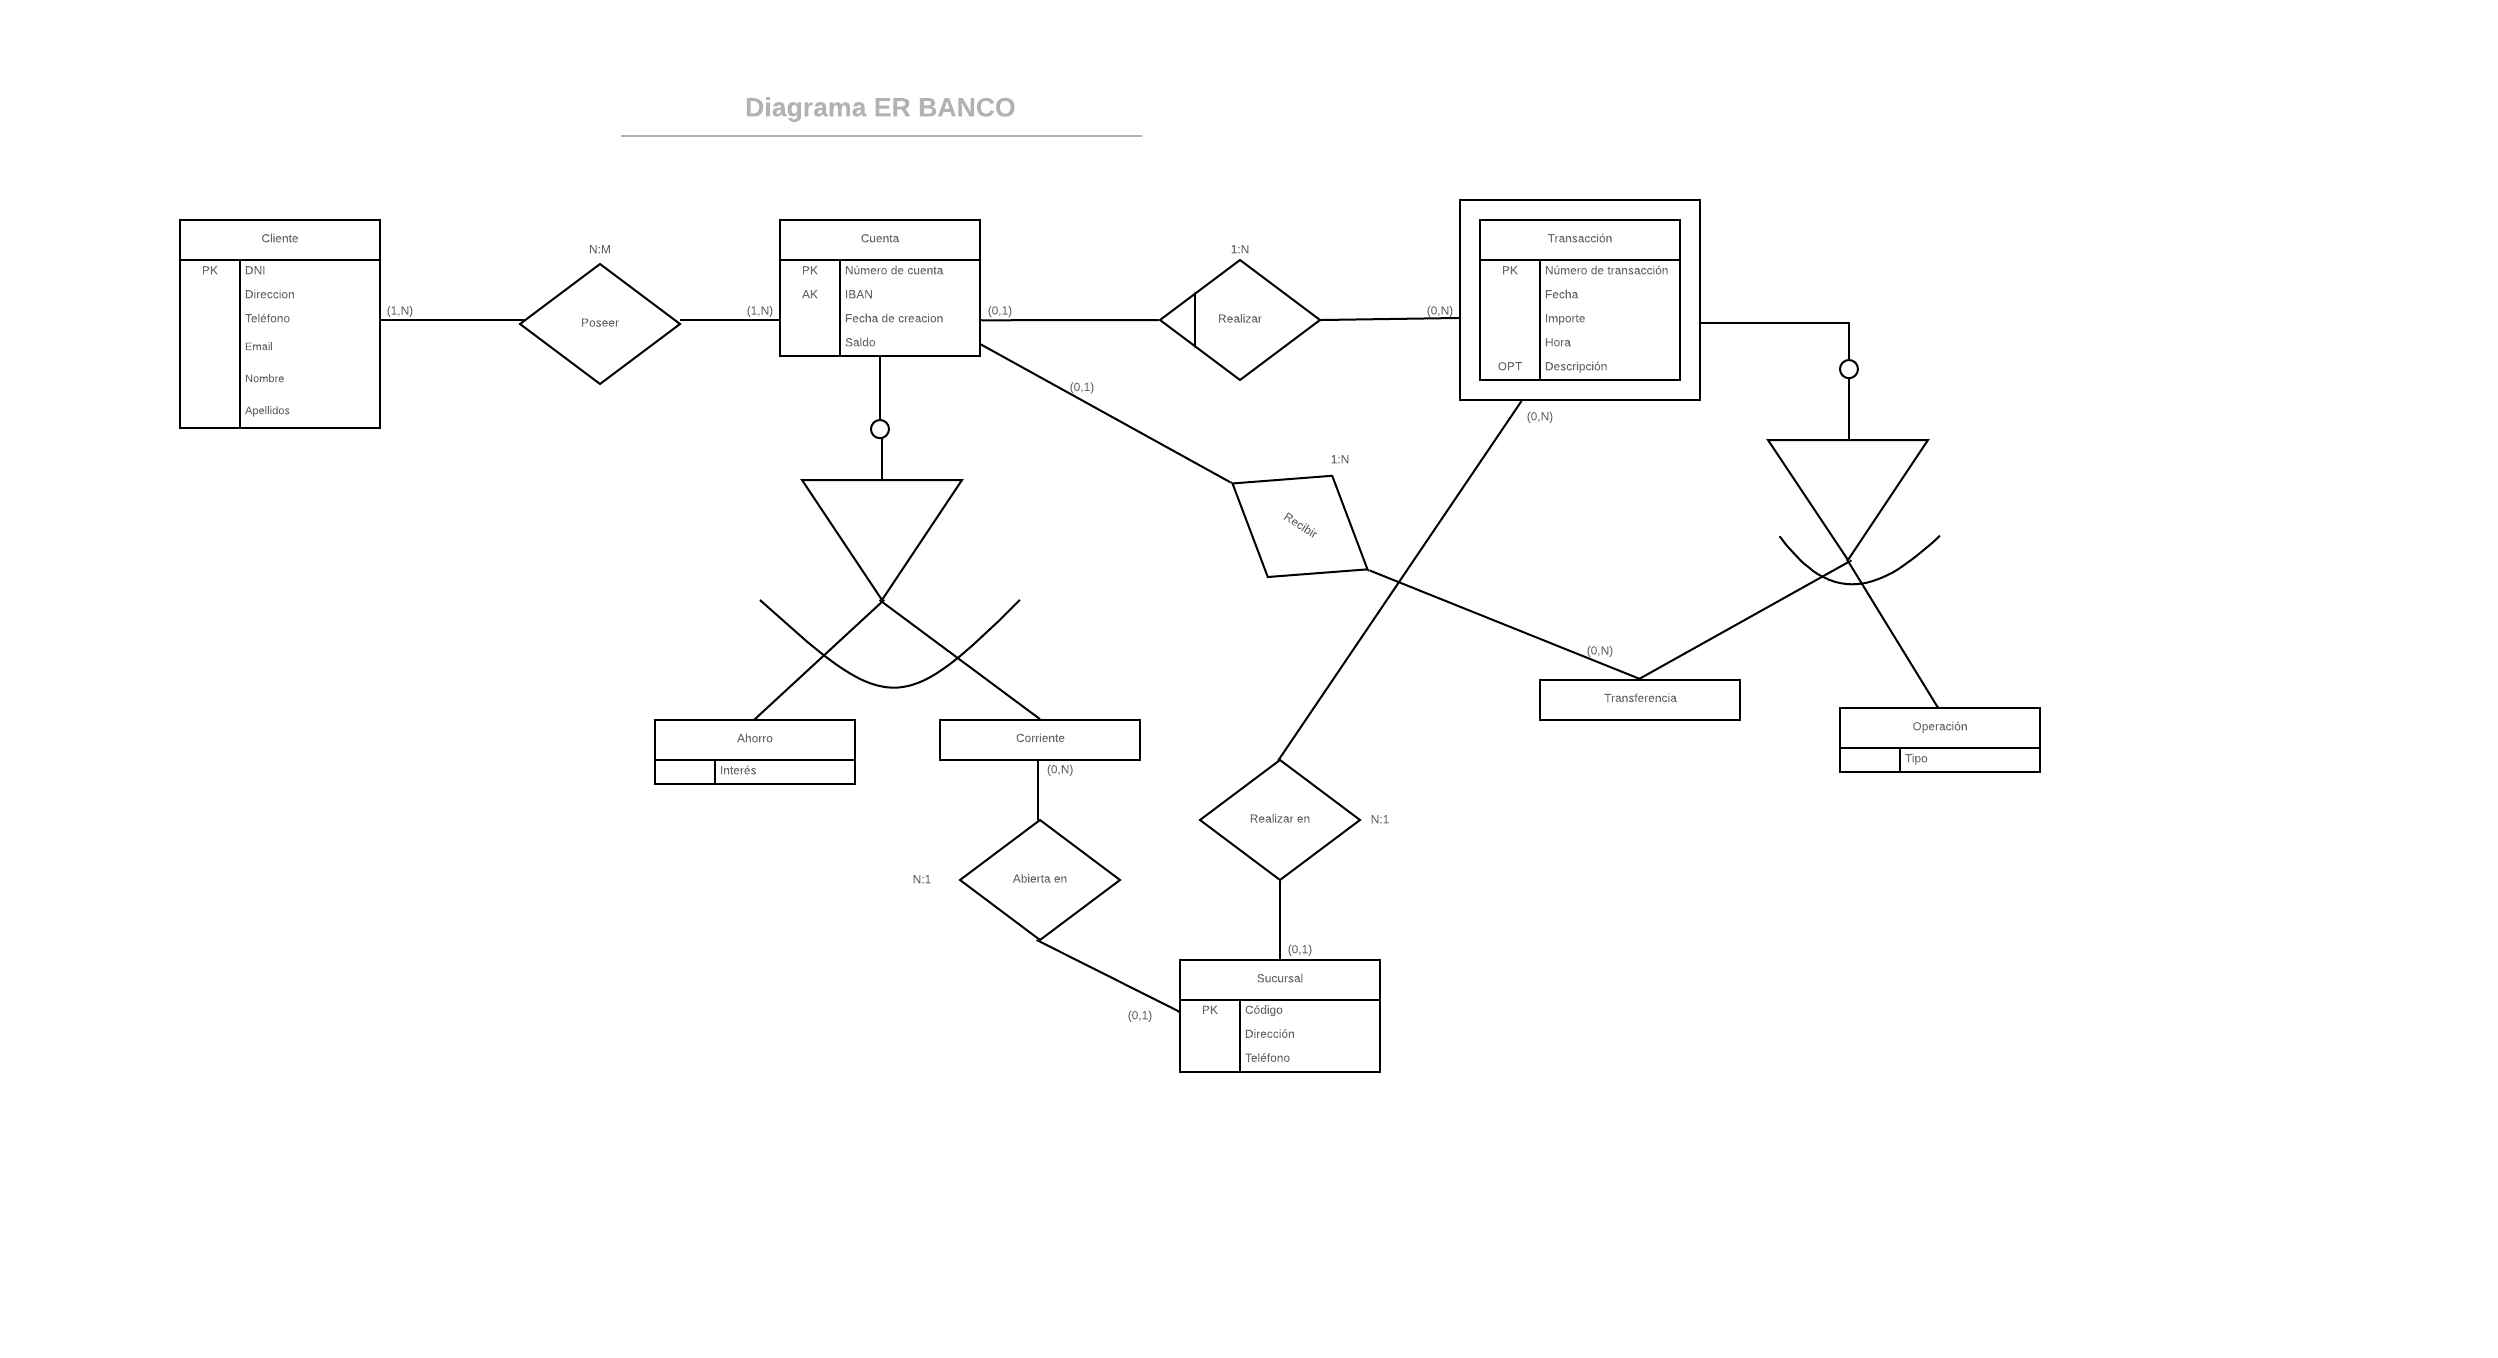
\includegraphics[scale=0.5]{images/diagramaer.png}
			\caption{Diagrama E-R de la Base de Datos a diseñar}
			\label{FIG:diagramaER}
\end{figure}

\begin{figure}[h!]
	\centering
		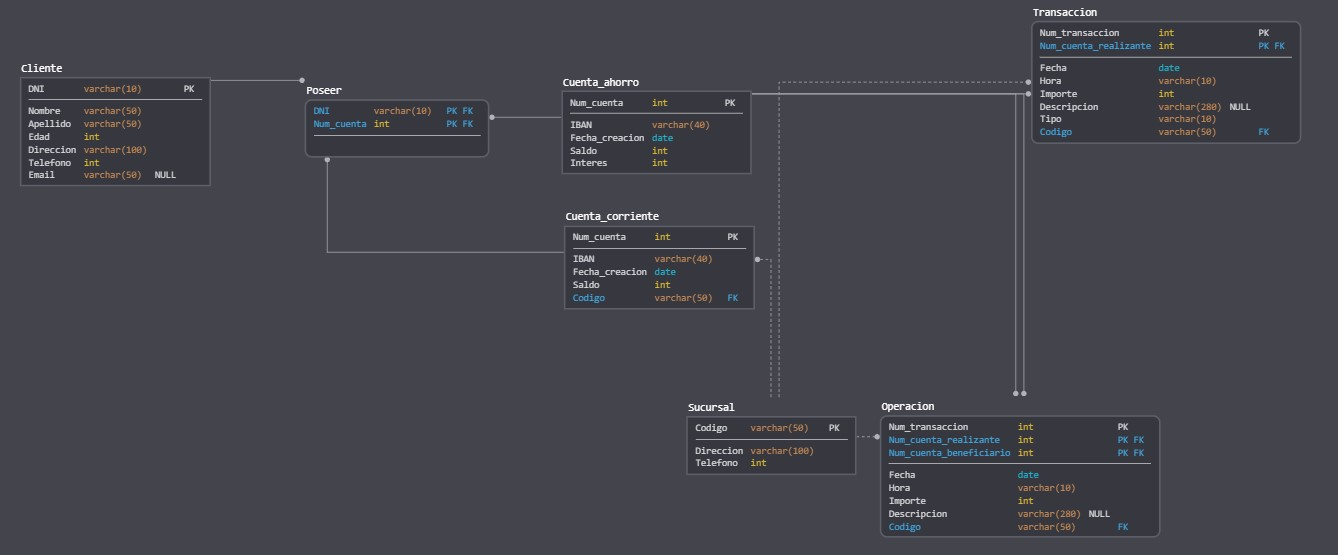
\includegraphics[scale=0.6]{images/diagramaRelacional.jpg}
			\caption{Diagrama del modelo relacional de la Base de Datos a diseñar}
			\label{FIG:diagramaRel}
\end{figure}

\begin{figure}[h!]
	\centering
		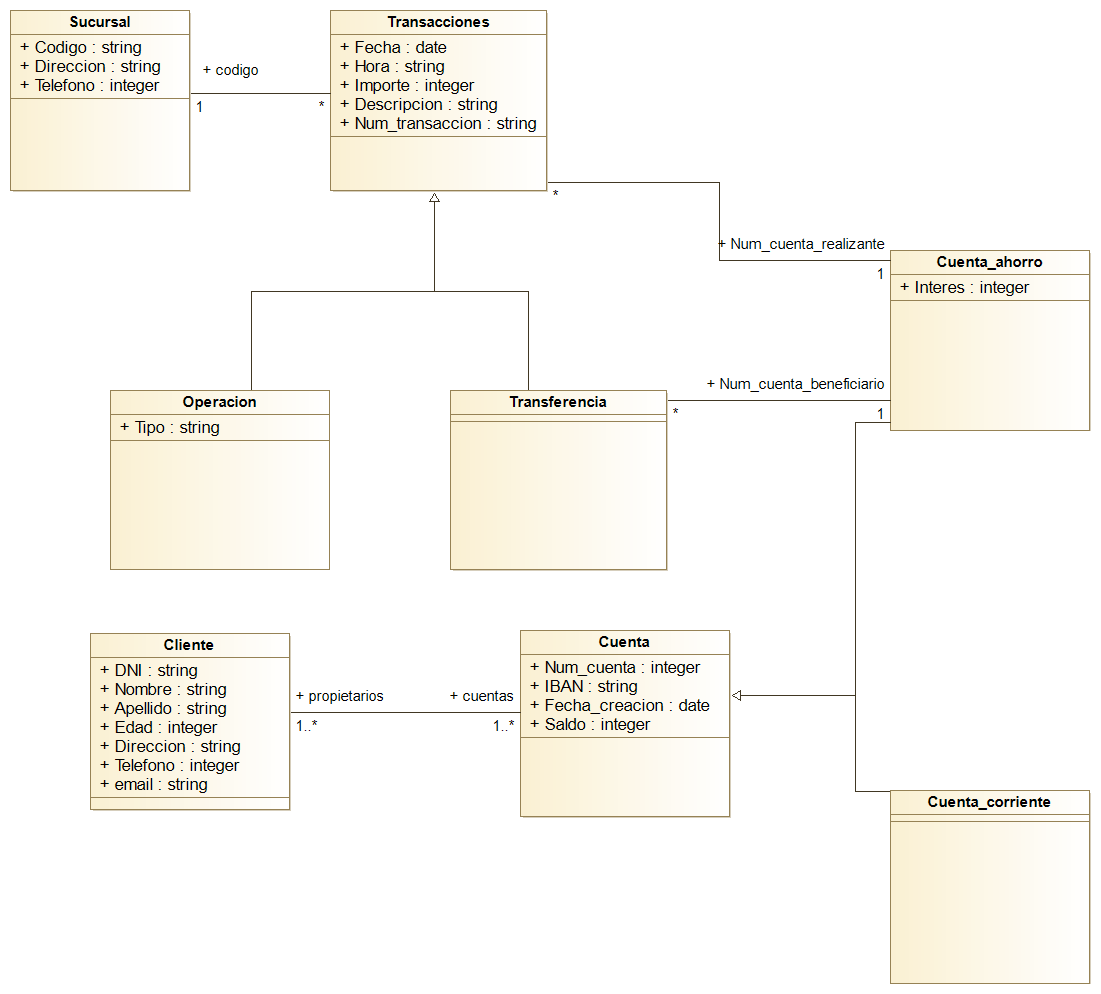
\includegraphics[scale=0.4]{images/diagramauml.png}
			\caption{Diagrama de clases UML de la Base de Datos a diseñar}
			\label{FIG:diagramaUML}
\end{figure}


\end{document}
